\clearpage
\thispagestyle{empty}
\section*{圣弗卢尔概率论暑期学校}

\begin{wrapfigure}{r}{.22\textwidth}
\centering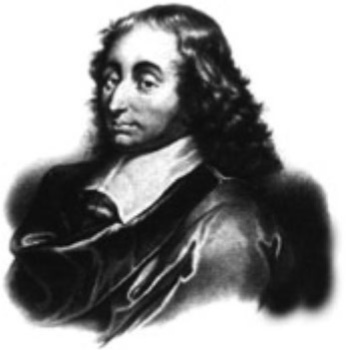
\includegraphics[width=.20\textwidth]{assets/front/saint-flour-portrait.png}
\end{wrapfigure}
圣弗卢尔系列卷册反映了圣弗卢尔概率论暑期学校的授课内容. 暑期学校创办于1971年，每年由法国克莱蒙费朗的布莱兹·帕斯卡数学实验室组织，该实验室隶属于法国国家科学研究中心（CNRS）和克莱蒙奥弗涅大学. 学校面向对概率论、统计学及其应用感兴趣的博士生、教师和研究人员.

学校持续12天（2005年以前为17天），最多接收100名参与者. 期间开设三门高水平课程，对概率论或统计学的某些领域作全面深入的研究. 讲师均由国际科学委员会选定. 参与者还有机会围绕自己的研究工作作简短报告.

参与者在同一栋建筑内住宿和学习. 这是一所位于圣弗卢尔市、建于18世纪的旧神学院，海拔900米. 宜人的环境有利于科学讨论与交流.

圣弗卢尔概率论暑期学校获得以下机构支持：
\begin{itemize}
\item 布莱兹·帕斯卡数学实验室；
\item 克莱蒙奥弗涅大学；
\item 法国国家科学研究中心（C.N.R.S.）；
\item 欧洲数学学会（E.M.S.）.
\end{itemize}
更多信息见：\url{https://lmbp.uca.fr/stflour/stflour-en.php}

\noindent\textbf{Christophe Bahadoran}\par
\href{mailto:Christophe.Bahadoran@uca.fr}{Christophe.Bahadoran@uca.fr}

\noindent\textbf{Arnaud Guillin}\par
\href{mailto:Arnaud.Guillin@uca.fr}{Arnaud.Guillin@uca.fr}

\noindent\textbf{Hacène Djellout}\par
\href{mailto:Hacene.Djellout@uca.fr}{Hacene.Djellout@uca.fr}

\href{mailto:stflour.lmbp@uca.fr}{stflour.lmbp@uca.fr}\par
法国克莱蒙奥弗涅大学，Aubière cedex
